% !TeX root = RJwrapper.tex
\title{Palmer Archipelago Penguins Data in the palmerpenguins R Package
- An Alternative to Anderson's Irises}
\author{by Allison M. Horst, Alison Presmanes Hill, and Kristen B. Gorman}

\maketitle

\abstract{%
In 1935, Edgar Anderson collected size measurements for 150 flowers from
three species of \emph{Iris} on the Gaspé Peninsula in Quebec, Canada.
Since then, Anderson's \emph{Iris} observations have become a classic
dataset in statistics, machine learning, and data science teaching
materials. It is included in the base R \CRANpkg{datasets} package as
\texttt{iris}, making it easy for users to access without knowing much
about it. However, the lack of data documentation, presence of
non-intuitive variables (e.g.~``sepal width''), and perfectly balanced
groups with zero missing values make \texttt{iris} an inadequate and
stale dataset for teaching and learning modern data science skills.
Users would benefit from working with a more representative, real-world
environmental dataset with a clear link to current scientific research.
Importantly, Anderson's \emph{Iris} data appeared in a 1936 publication
by R. A. Fisher in the \emph{Annals of Eugenics} (which is often the
first-listed citation for the dataset), inextricably linking
\texttt{iris} to eugenics research. Thus, a modern alternative to
\texttt{iris} is needed. In this paper, we introduce the
\CRANpkg{palmerpenguins} R package \citep{R-palmerpenguins}, which
includes body size measurements collected from 2007 - 2009 for three
species of \emph{Pygoscelis} penguins that breed on islands throughout
the Palmer Archipelago, Antarctica. The \texttt{penguins} dataset in
\CRANpkg{palmerpenguins} provides an approachable, charismatic, and near
drop-in replacement for \texttt{iris} with topical relevance for polar
climate change and environmental impacts on marine predators. Since the
release on CRAN in July 2020, the \CRANpkg{palmerpenguins} package has
been downloaded over 462,000 times, highlighting the demand and
widespread adoption of this viable \texttt{iris} alternative. We
directly compare the \texttt{iris} and \texttt{penguins} datasets for
selected analyses to demonstrate that R users, in particular teachers
and learners currently using \texttt{iris}, can switch to the Palmer
Archipelago penguins for many use cases including data wrangling,
visualization, linear modeling, multivariate analysis (e.g., PCA),
cluster analysis and classification (e.g., by k-means).
}

\hypertarget{introduction}{%
\subsection{Introduction}\label{introduction}}

In 1935, American botanist Edgar Anderson measured petal and sepal
structural dimensions (length and width) for 50 flowers from three
\emph{Iris} species: \emph{Iris setosa}, \emph{Iris versicolor}, and
\emph{Iris virginica} \citep{anderson_irises_1935}. The manageable but
non-trivial size (5 variables and 150 total observations) and
characteristics of Anderson's \emph{Iris} dataset, including linear
relationships and multivariate normality, have made it amenable for
introducing a wide range of statistical methods including data
wrangling, visualization, linear modeling, multivariate analyses, and
machine learning. The \emph{Iris} dataset is built into a number of
software packages including the auto-installed datasets package in R
\citep[as \texttt{iris},][]{R-base}, Python's scikit-learn machine
learning library \citep{pedregosa_scikit-learn_2011}, and the SAS
Sashelp library (SAS Institute, Cary NC), which has facilitated its
widespread use. As a result, eighty-six years after the data were
initially published, the \emph{Iris} dataset remains ubiquitous in
statistics, computational methods, software documentation, and data
science courses and materials.

There are a number of reasons that modern data science practitioners and
educators may want to move on from \texttt{iris}. First, the dataset
lacks metadata \citep{anderson_irises_1935}, which does not reinforce
best practices and limits meaningful interpretation and discussion of
research methods, analyses, and outcomes. Of the five variables in
\texttt{iris}, two (\texttt{Sepal.Width} and \texttt{Sepal.Length}) are
not intuitive for most non-botanists. Even with explanation, the
difference between \emph{petal} and \emph{sepal} dimensions is not
obvious. Second, \texttt{iris} contains equal sample sizes for each of
the three species (\emph{n} = 50) with no missing values, which is
cleaner than most real-world data that learners are likely to encounter.
Third, the single factor (\texttt{Species}) in \texttt{iris} limits
options for analyses. Finally, due to its publication in the
\emph{Annals of Eugenics} by statistician R.A. Fisher
\citep{fisher_use_1936}, \texttt{iris} is burdened by a history in
eugenics research, which we are committed to addressing through the
development of new data science education products as described below.

Given the growing need for fresh data science-ready datasets, we sought
to identify an alternative dataset that could be made easily accessible
for a broad audience. After evaluating the positive and negative
features of \texttt{iris} in data science and statistics materials, we
established the following criteria for a suitable alternative:

\begin{itemize}
\tightlist
\item
  Available by appropriate license like a
  \href{https://creativecommons.org/share-your-work/public-domain/cc0/}{Creative
  Commons 0 license} (CC0 ``no rights reserved'')
\item
  Feature intuitive subjects and variables that are interesting and
  understandable to learners across disciplines
\item
  Complete metadata and documentation
\item
  Manageable (but not trivial) in size
\item
  Minimal data cleaning and pre-processing required for most analyses
\item
  Real-world (not manufactured) modern data
\item
  Provides similar opportunities for teaching and learning R, data
  science, and statistical skills
\item
  Can easily replace \texttt{iris} for most use cases
\end{itemize}

Here, we describe an alternative to \texttt{iris} that largely satisfies
these criteria: a refreshing, approachable, and charismatic dataset
containing real-world body size measurements for three \emph{Pygoscelis}
penguin species that breed throughout the Western Antarctic Peninsula
region, made available through the United States Long-Term Ecological
Research (US LTER) Network. By comparing data structure, size, and a
range of analyses side-by-side for the two datasets, we demonstrate that
the Palmer Archipelago penguin data are an ideal substitute for
\texttt{iris} for many use cases in statistics and data science
education.

\hypertarget{data-source}{%
\subsection{Data source}\label{data-source}}

Body size measurements (bill length and depth, flipper length - flippers
are the modified ``wings'' of penguins used for maneuvering in water,
and body mass), clutch (i.e., egg laying) observations (e.g., date of
first egg laid, and clutch completion), and carbon
(\textsuperscript{13}C/\textsuperscript{12}C,
\(\delta\)\textsuperscript{13}C) and nitrogen
(\textsuperscript{15}N/\textsuperscript{14}N,
\(\delta\)\textsuperscript{15}N) stable isotope values of red blood
cells for adult male and female Adélie (\emph{P. adeliae}), chinstrap
(\emph{P. antarcticus}), and gentoo (\emph{P. papua}) penguins on three
islands (Biscoe, Dream, and Torgersen) within the Palmer Archipelago
were collected from 2007 - 2009 by Dr.~Kristen Gorman in collaboration
with the \href{https://pal.lternet.edu/}{Palmer Station LTER}, part of
the \href{https://lternet.edu/}{US LTER Network}. For complete data
collection methods and published analyses, see
\citet{gorman_ecological_2014}. Throughout this paper, penguins species
are referred to as ``Adélie'', ``Chinstrap'', and ``Gentoo''.

The data in the \CRANpkg{palmerpenguins} R package are available for use
by CC0 license (``No Rights Reserved'') in accordance with the
\href{https://pal.lternet.edu/data/policies}{Palmer Station LTER Data
Policy} and the \href{https://lternet.edu/data-access-policy/}{LTER Data
Access Policy}, and were imported from the
\href{https://environmentaldatainitiative.org/}{Environmental Data
Initiative (EDI) Data Portal} at the links below:

\begin{itemize}
\tightlist
\item
  Adélie penguin data
  \citep{palmer_station_antarctica_lter_structural_2020}:
  \href{https://portal.edirepository.org/nis/mapbrowse?packageid=knb-lter-pal.219.5}{KNB-LTER
  Data Package 219.5}
\item
  Gentoo penguin data
  \citep{palmer_station_antarctica_lter_structural_2020-1}:
  \href{https://portal.edirepository.org/nis/mapbrowse?packageid=knb-lter-pal.220.5}{KNB-LTER
  Data Package 220.5}
\item
  Chinstrap penguin data
  \citep{palmer_station_antarctica_lter_structural_2020-2}:
  \href{https://portal.edirepository.org/nis/mapbrowse?packageid=knb-lter-pal.221.6}{KNB-LTER
  Data Package 221.6}
\end{itemize}

\hypertarget{the-palmerpenguins-r-package}{%
\subsection{The palmerpenguins R
package}\label{the-palmerpenguins-r-package}}

R users can install the \CRANpkg{palmerpenguins} package from CRAN:

\begin{verbatim}
install.packages("palmerpenguins")
\end{verbatim}

Information, examples, and links to community-contributed materials are
available on the \CRANpkg{palmerpenguins} package website:
\href{https://allisonhorst.github.io/palmerpenguins/}{allisonhorst.github.io/palmerpenguins/}.
See the Appendix for how Python and Julia users can access the same
data.

The \CRANpkg{palmerpenguins} R package contains two data objects:
\texttt{penguins\_raw} and \texttt{penguins}. The \texttt{penguins\_raw}
data consists of all raw data for 17 variables, recorded completely or
in part for 344 individual penguins, accessed directly from EDI
(\texttt{penguins\_raw} properties are summarized in Appendix B). We
generally recommend using the curated data in \texttt{penguins}, which
is a subset of \texttt{penguins\_raw} retaining all 344 observations,
minimally updated (Appendix A) and reduced to the following eight
variables:

\begin{itemize}
\tightlist
\item
  \texttt{species}: a factor denoting the penguin species (Adélie,
  Chinstrap, or Gentoo)
\item
  \texttt{island}: a factor denoting the Palmer Archipelago island in
  Antarctica where each penguin was observed (Biscoe Point, Dream
  Island, or Torgersen Island)
\item
  \texttt{bill\_length\_mm}: a number denoting length of the dorsal
  ridge of a penguin bill (millimeters)
\item
  \texttt{bill\_depth\_mm}: a number denoting the depth of a penguin
  bill (millimeters)
\item
  \texttt{flipper\_length\_mm}: an integer denoting the length of a
  penguin flipper (millimeters)
\item
  \texttt{body\_mass\_g}: an integer denoting the weight of a penguin's
  body (grams)
\item
  \texttt{sex}: a factor denoting the sex of a penguin sex (male,
  female) based on molecular data
\item
  \texttt{year}: an integer denoting the year of study (2007, 2008, or
  2009)
\end{itemize}

The same data exist as comma-separated value (CSV) files in the package
(``penguins\_raw.csv'' and ``penguins.csv''), and can be read in using
the built-in \texttt{path\_to\_file()} function in
\CRANpkg{palmerpenguins}. For example,

\begin{verbatim}
library(palmerpenguins)
df <- read.csv(path_to_file("penguins.csv"))
\end{verbatim}

will read in ``penguins.csv'' as if from an external file, thus
automatically parsing \texttt{species}, \texttt{island}, and
\texttt{sex} variables as characters instead of factors. This option
allows users opportunities to practice or demonstrate reading in data
from a CSV, then updating variable class (e.g., characters to factors).

\hypertarget{comparing-iris-and-penguins}{%
\subsection{\texorpdfstring{Comparing \texttt{iris} and
\texttt{penguins}}{Comparing iris and penguins}}\label{comparing-iris-and-penguins}}

The \texttt{penguins} data in \CRANpkg{palmerpenguins} is useful and
approachable for data science and statistics education, and is uniquely
well-suited to replace the \texttt{iris} dataset. Comparisons presented
are selected examples for common \texttt{iris} uses, and are not
exhaustive.

\begin{Schunk}
\begin{table}

\caption{\label{tab:overview-tbl-pdf}Overview comparison of \textbf{penguins} and \textbf{iris} dataset features and characteristics.}
\centering
\begin{tabular}[t]{lcl}
\toprule
Feature & iris & penguins\\
\midrule
Year(s) collected & 1935 & 2007 - 2009\\
Dimensions (col x row) & 5 x 150 & 8 x 344\\
Documentation & minimal & complete metadata\\
Variable classes & double (4), factor (1) & double (2), int (3), factor (3)\\
Missing values? & no (n = 0; 0.0\%) & yes (n = 19; 0.7\%)\\
\bottomrule
\end{tabular}
\end{table}

\end{Schunk}

\hypertarget{data-structure-and-sample-size}{%
\subsubsection{Data structure and sample
size}\label{data-structure-and-sample-size}}

Both \texttt{iris} and \texttt{penguins} are in tidy format
\citep{wickham_tidy_2014} with each column denoting a single variable
and each row containing measurements for a single iris flower or
penguin, respectively. The two datasets are comparable in size:
dimensions (columns × rows) are 5 × 150 and 8 × 344 for \texttt{iris}
and \texttt{penguins}, respectively, and sample sizes within species are
similar (Tables \ref{tab:overview-tbl} \& \ref{tab:counts-tbl}).

Notably, while sample sizes in \texttt{iris} across species are all the
same, sample sizes in \texttt{penguins} differ across the three species.
The inclusion of three factor variables in \texttt{penguins}
(\texttt{species}, \texttt{island}, and \texttt{sex}), along with
\texttt{year}, create additional opportunities for grouping, faceting,
and analysis compared to the single factor (\texttt{Species}) in
\texttt{iris}.

Unlike \texttt{iris}, which contains only complete cases, the
\texttt{penguins} dataset contains a small number of missing values
(\emph{n}\textsubscript{missing} = 19, out of 2,752 total values).
Missing values and unequal sample sizes are common in real-world data,
and create added learning opportunity to the \texttt{penguins} dataset.

\begin{Schunk}
\begin{table}

\caption{\label{tab:counts-tbl-pdf}Grouped sample size for \textbf{iris} (by species; \textit{n} = 150 total) and \textbf{penguins} (by species and sex; \textit{n} = 344 total). Data in \textbf{penguins} can be further grouped by island and study year.}
\centering
\begin{tabular}[t]{lclccc}
\toprule
\multicolumn{2}{c}{iris sample size (by species)} & \multicolumn{4}{c}{penguins sample size (by species and sex)} \\
\cmidrule(l{3pt}r{3pt}){1-2} \cmidrule(l{3pt}r{3pt}){3-6}
Iris species & Sample size & Penguin species & Female & Male & NA\\
\midrule
setosa & 50 & Adélie & 73 & 73 & 6\\
versicolor & 50 & Chinstrap & 34 & 34 & 0\\
virginica & 50 & Gentoo & 58 & 61 & 5\\
\bottomrule
\end{tabular}
\end{table}

\end{Schunk}

\hypertarget{continuous-quantitative-variables}{%
\subsubsection{Continuous quantitative
variables}\label{continuous-quantitative-variables}}

Distributions, relationships between variables, and clustering can be
visually explored between species for the four structural size
measurements in \texttt{penguins} (flipper length, body mass, bill
length and depth; Figure \ref{fig:penguin-pairs}) and \texttt{iris}
(sepal width and length, petal width and length; Figure
\ref{fig:iris-pairs}).

\begin{Schunk}
\begin{figure}[htbp]

{\centering 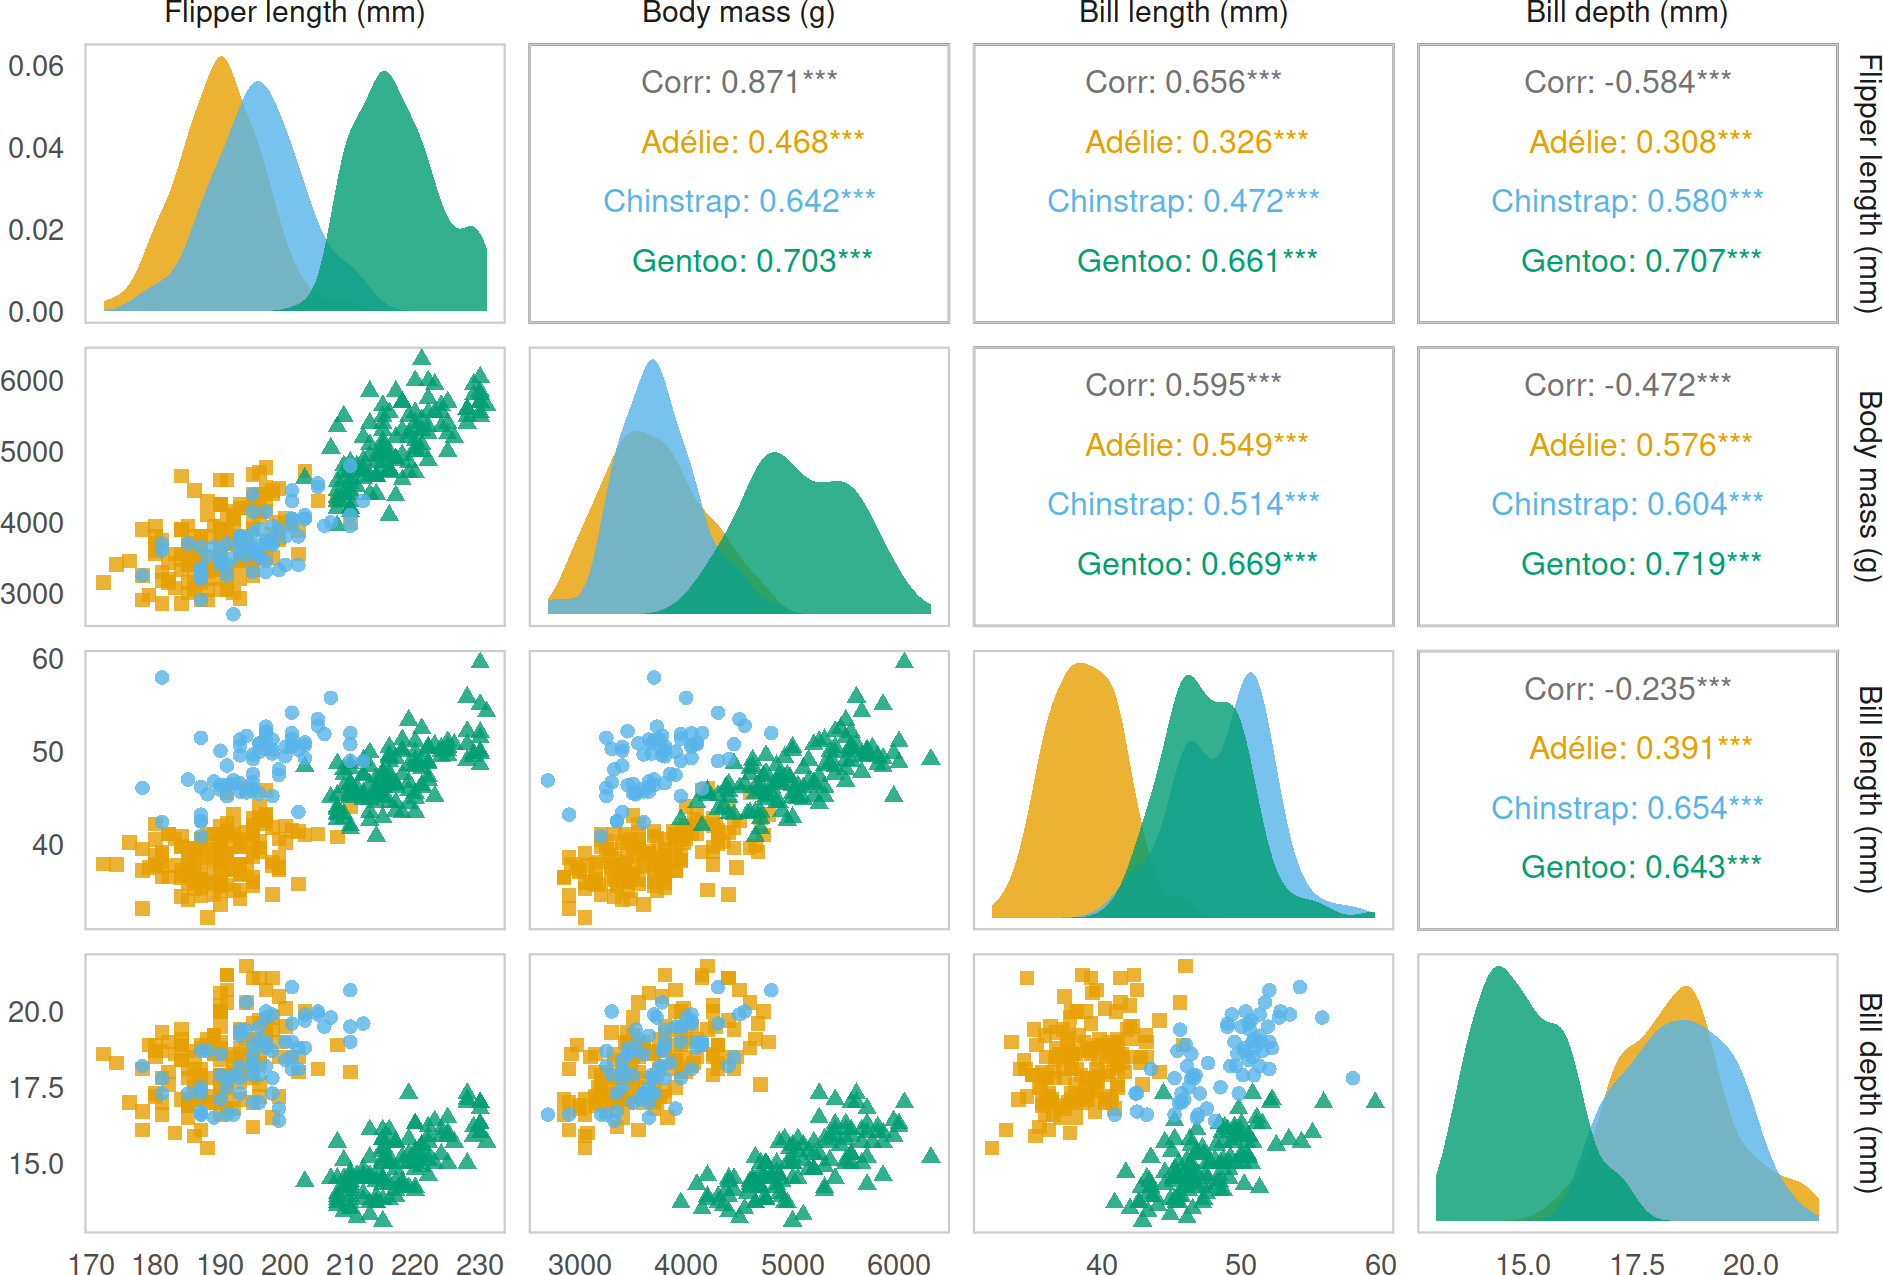
\includegraphics[width=\textwidth]{figs/penguin-pairs-1} 

}

\caption{Distributions and correlations for numeric variables in the \textbf{penguins} data (flipper length (mm), body mass (g), bill length (mm) and bill depth (mm)) for the three observed species: Gentoo (green, triangles); Chinstrap (blue, circles); and Adélie (orange, squares). Significance indicated for bivariate correlations: \text{*}\textit{p} < 0.05; \text{*}\text{*}\textit{p} < 0.01; \text{*}\text{*}\text{*}\textit{p} < 0.001.}\label{fig:penguin-pairs}
\end{figure}
\end{Schunk}

\begin{Schunk}
\begin{figure}[htbp]

{\centering 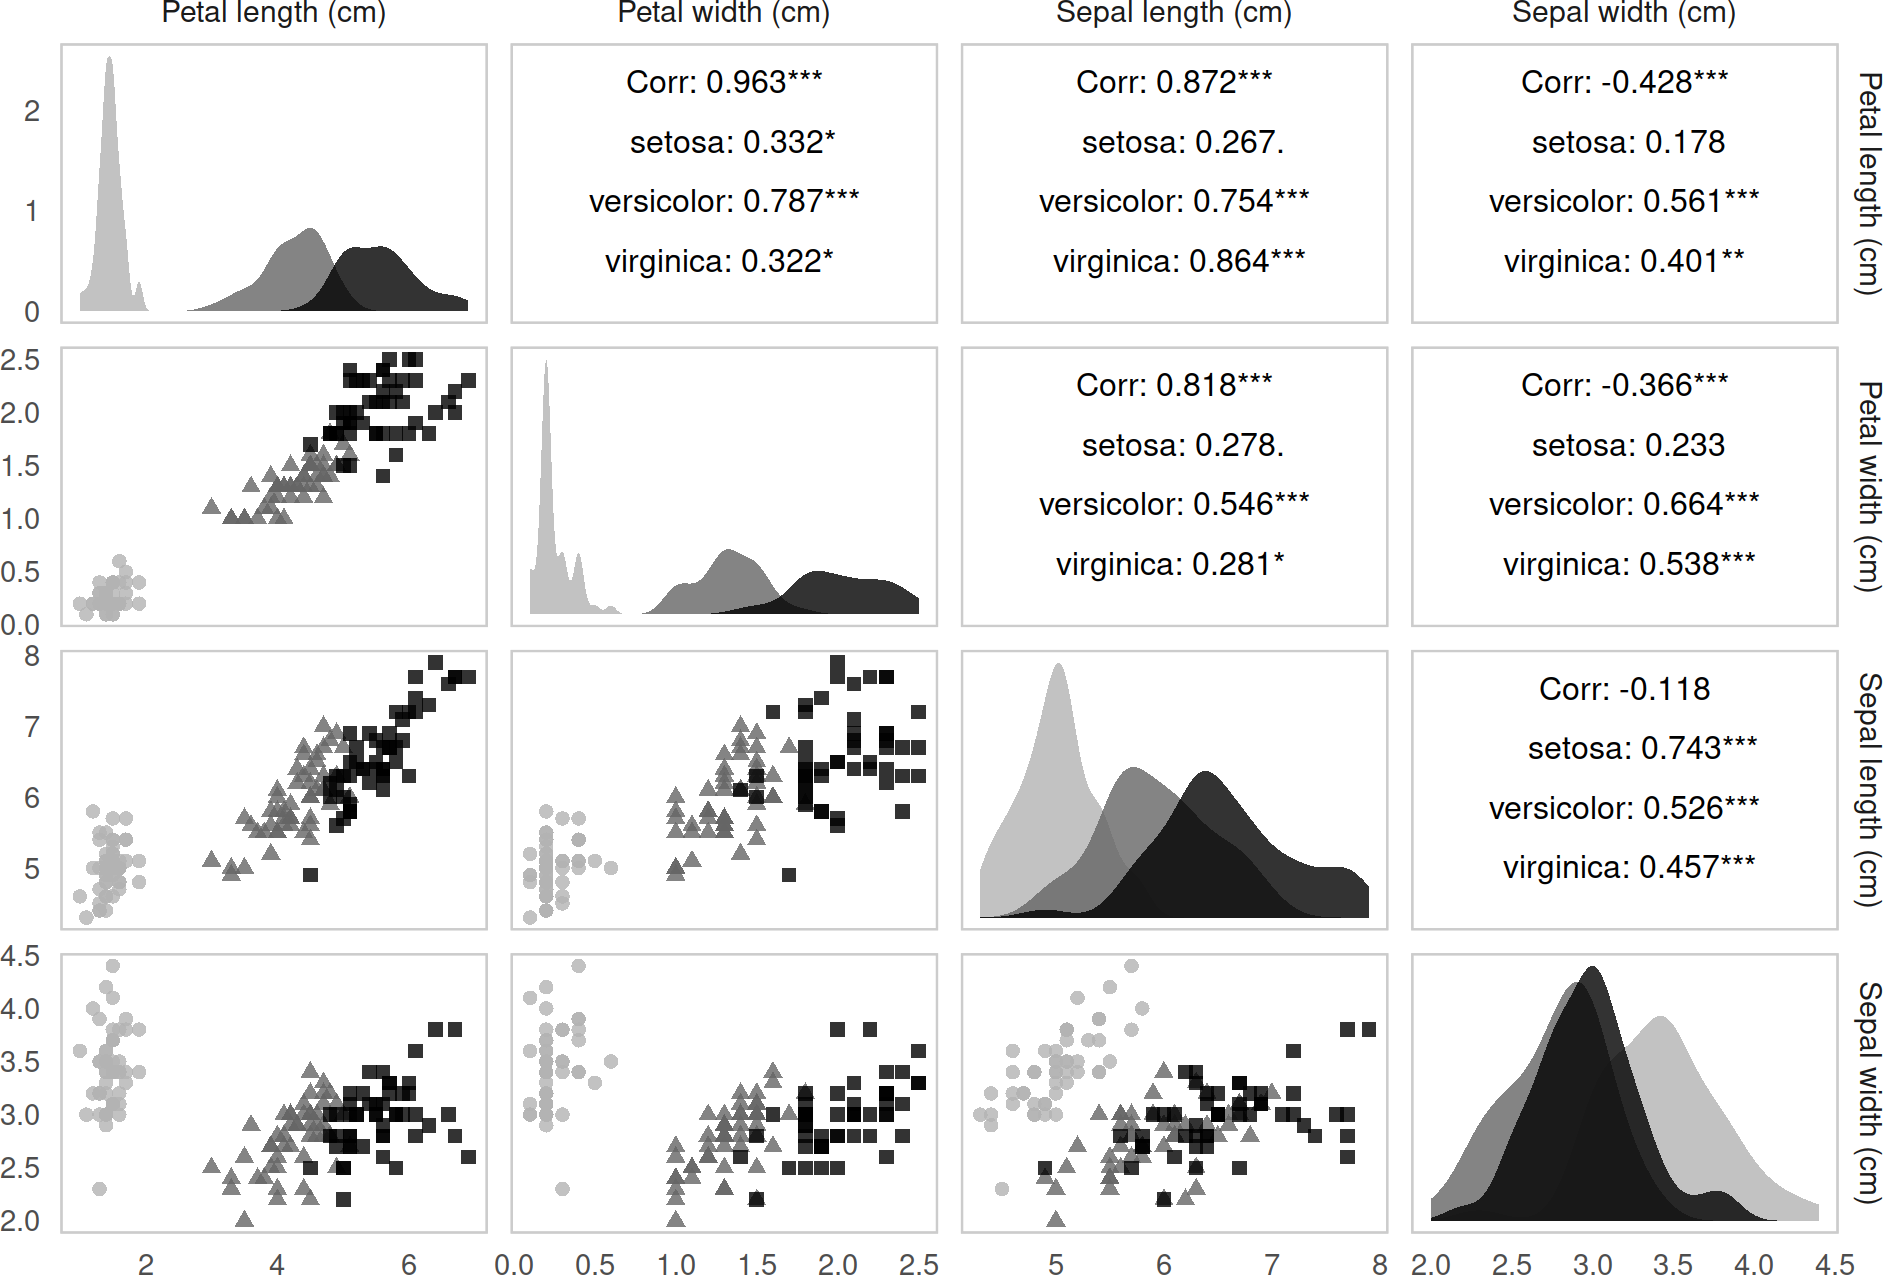
\includegraphics[width=\textwidth]{figs/iris-pairs-1} 

}

\caption{Distributions and correlations for numeric variables in \textbf{iris} (petal length (cm), petal width (cm), sepal length (cm) and sepal width (cm)) for the three included iris species: \textit{Iris setosa} (light gray, circles); \textit{Iris versicolor} (dark gray, triangles); and \textit{Iris virginica} (black, squares). Significance indicated for bivariate correlations: \text{*}\textit{p} < 0.05; \text{*}\text{*}\textit{p} < 0.01; \text{*}\text{*}\text{*}\textit{p} < 0.001.}\label{fig:iris-pairs}
\end{figure}
\end{Schunk}

Both \texttt{penguins} and \texttt{iris} offer numerous opportunities to
explore linear relationships and correlations, within and across species
(Figures \ref{fig:penguin-pairs} \& \ref{fig:iris-pairs}). A bivariate
scatterplot made with the \texttt{iris} dataset reveals a clear linear
relationship between petal length and petal width. Using
\texttt{penguins} (Figure \ref{fig:linear}), we can create a uniquely
similar scatterplot with flipper length and body mass. The overall trend
across all three species is approximately linear for both \texttt{iris}
and \texttt{penguins}. Teachers may encourage students to explore how
simple linear regression results and predictions differ when the species
variable is omitted, compared to, for example, multiple linear
regression with species included (Figure \ref{fig:linear}).

\begin{Schunk}
\begin{figure}[htbp]

{\centering 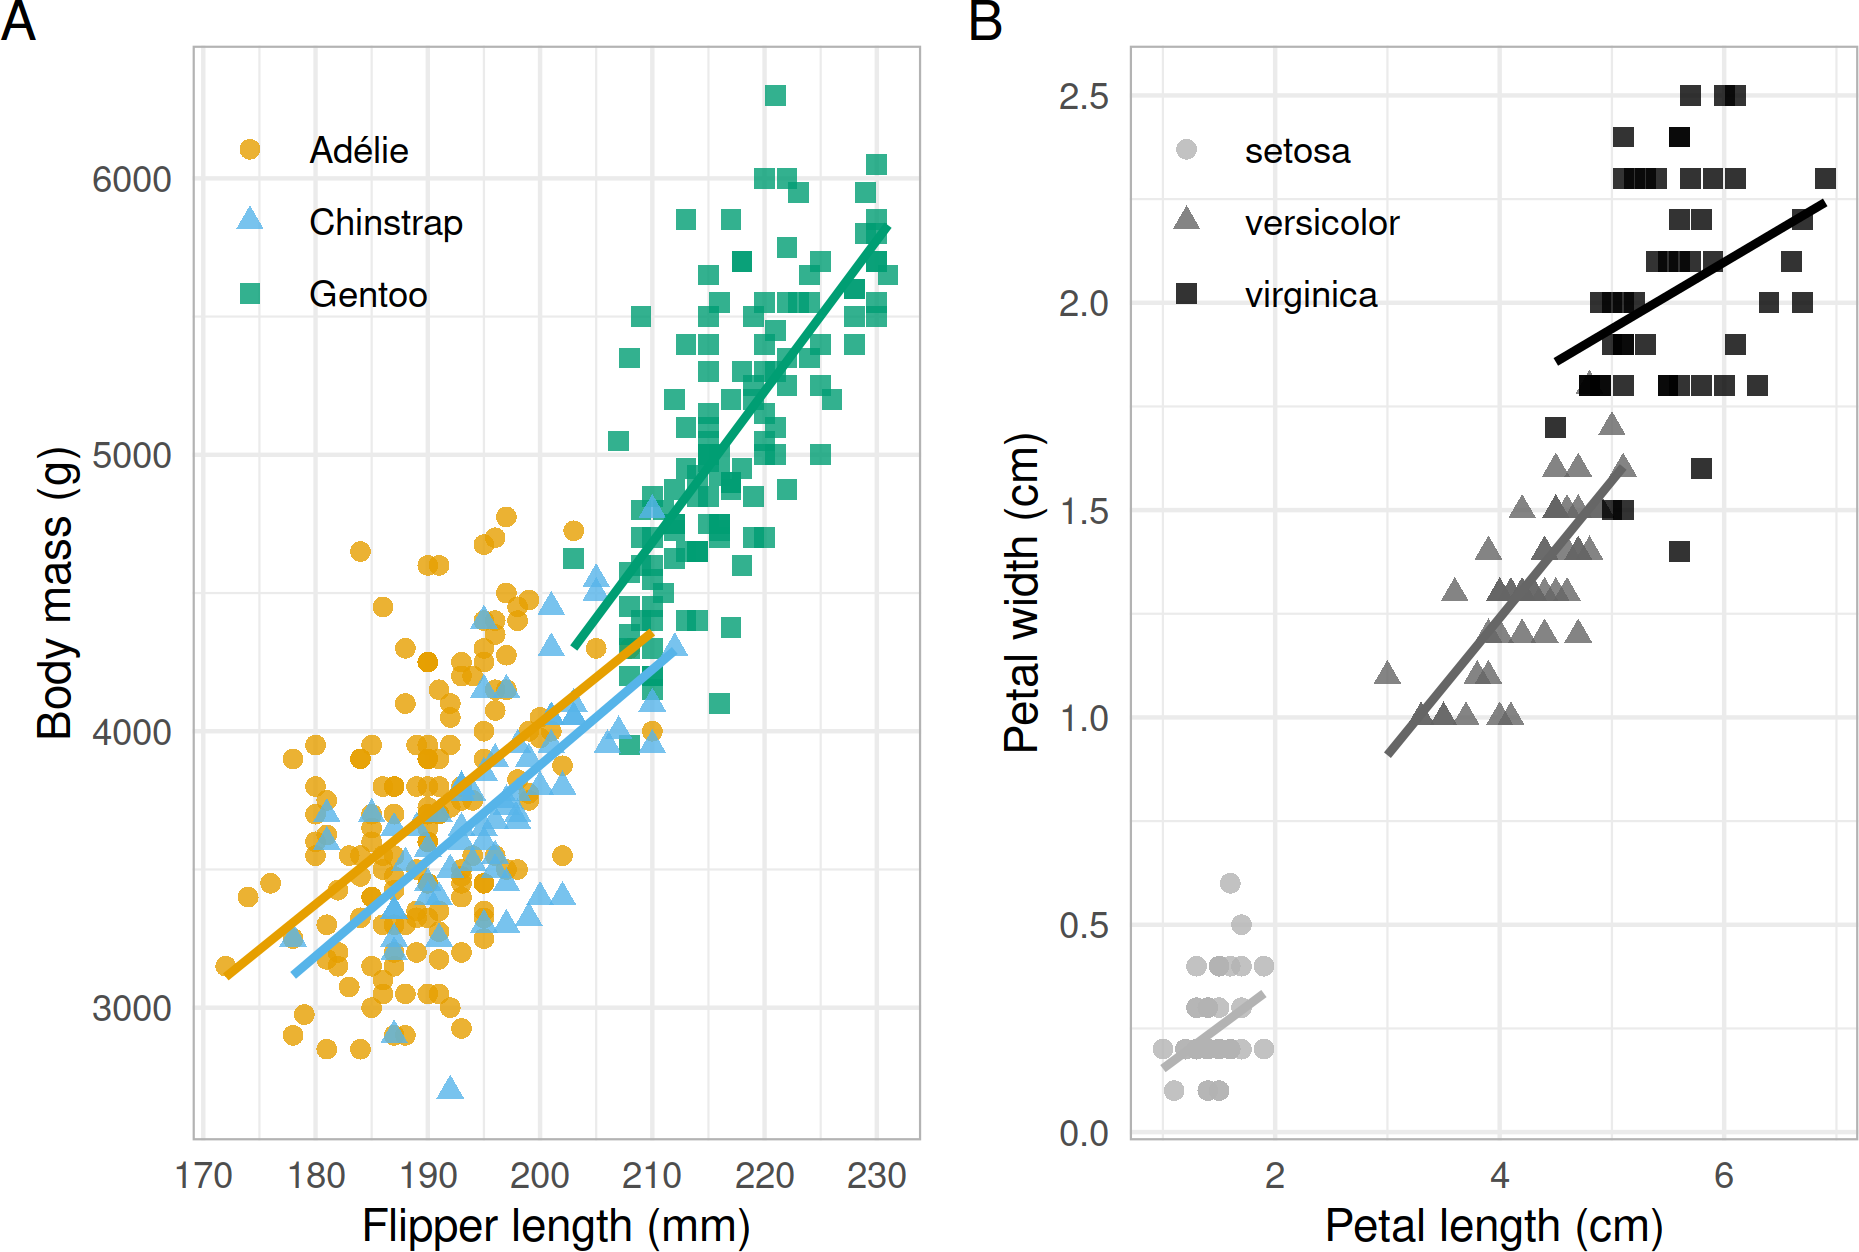
\includegraphics[width=\textwidth]{figs/linear-1} 

}

\caption[Representative linear relationships for (A)]{Representative linear relationships for (A): penguin flipper length (mm) and body mass (g) for Adélie (orange circles), Chinstrap (blue triangles), and Gentoo (green squares) penguins; (B): iris petal length (cm) and width (cm) for \textit{Iris setosa} (light gray circles), \textit{Iris versicolor} (dark gray triangles) and \textit{Iris virginica} (black squares). Within-species linear model is visualized for each penguin or iris species.}\label{fig:linear}
\end{figure}
\end{Schunk}

Notably, distinctions between species are clearer for iris petals -
particularly, the much smaller petals for \emph{Iris setosa} - compared
to penguins, in which Adélie and Chinstrap penguins are largely
overlapping in body size (body mass and flipper length), and are both
generally smaller than Gentoo penguins.

Simpson's Paradox is a data phenomenon in which a trend observed between
variables is reversed when data are pooled, omitting a meaningful
variable. While often taught and discussed in statistics courses,
finding a real-world and approachable example of Simpson's Paradox can
be a challenge. Here, we show one (of several possible - see Figure
\ref{fig:penguin-pairs}) Simpson's Paradox example in \texttt{penguins}:
exploring bill dimensions with and without species included (Figure
\ref{fig:simpsons}). When penguin species is omitted (Figure
\ref{fig:simpsons}A), bill length and depth appear negatively correlated
overall. The trend is reversed when species is included, revealing an
obviously positive correlation between bill length and bill depth within
species (Figure \ref{fig:simpsons}B).

\begin{Schunk}
\begin{figure}[htbp]

{\centering 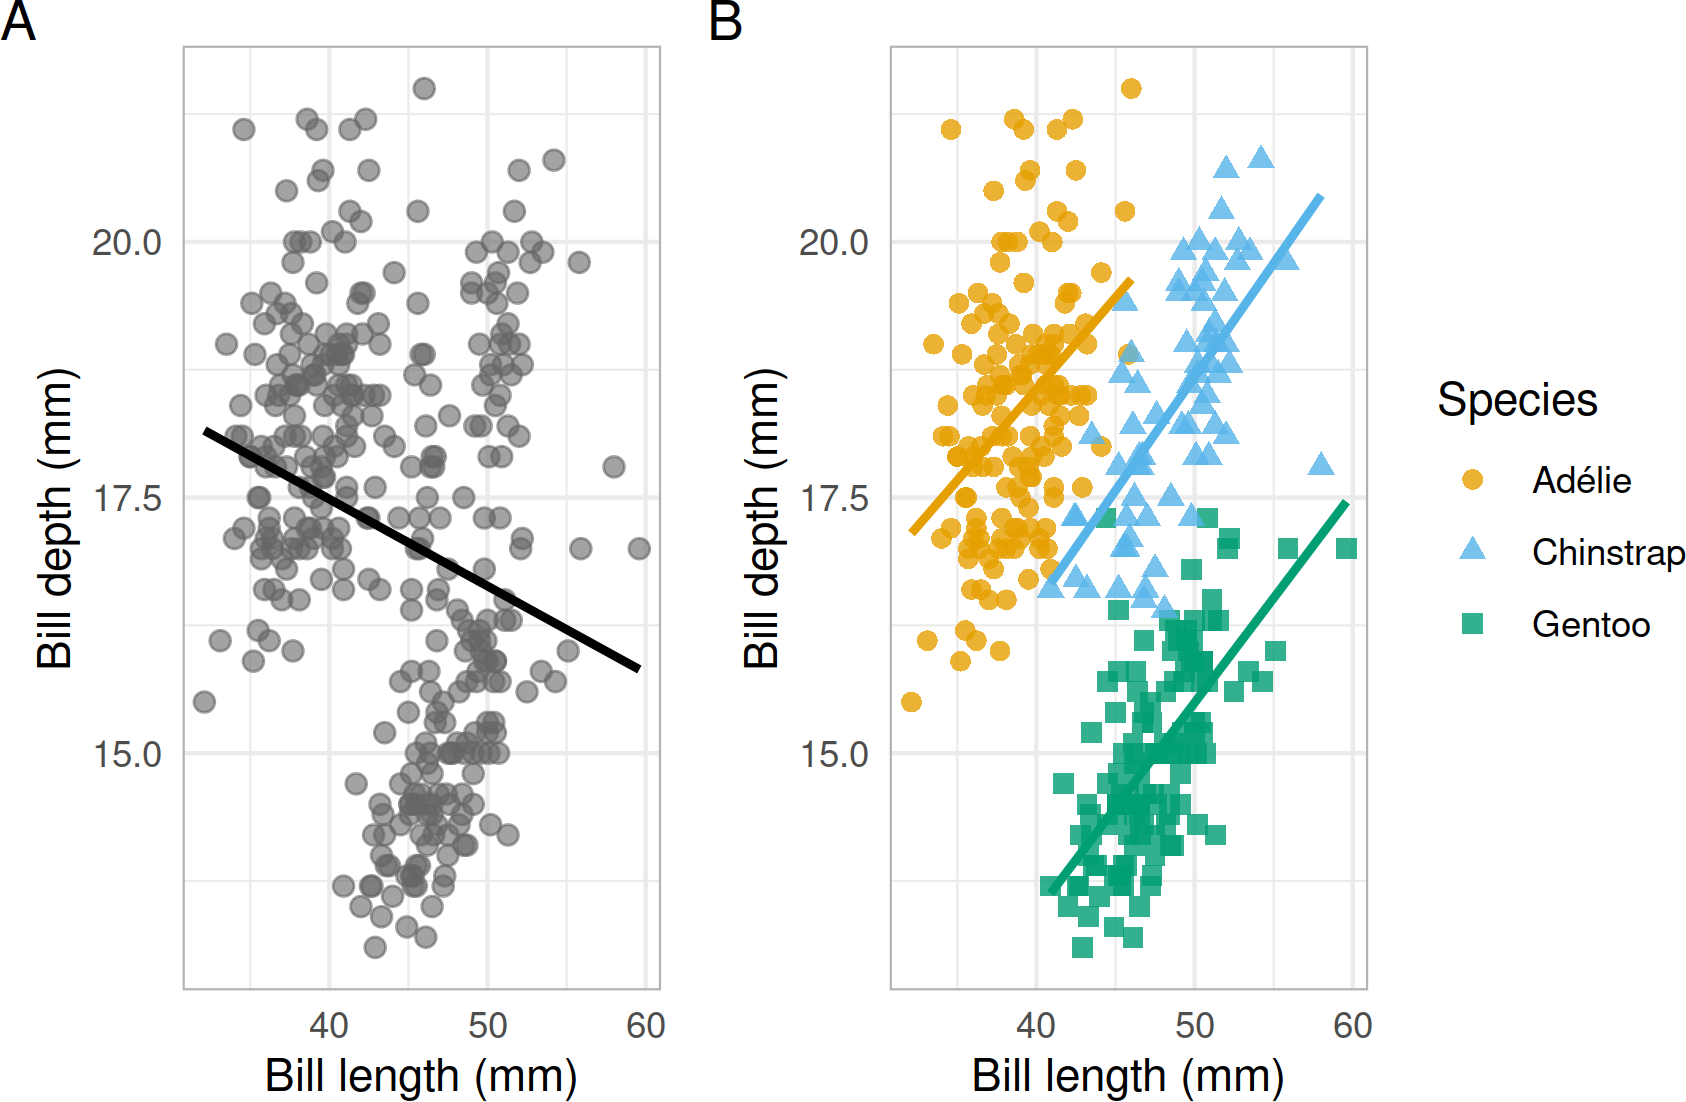
\includegraphics[width=\textwidth]{figs/simpsons-1} 

}

\caption[Trends for penguin bill dimensions (bill length and bill depth, millimeters) if the species variable is excluded (A) or included (B), illustrating Simpson’s Paradox]{Trends for penguin bill dimensions (bill length and bill depth, millimeters) if the species variable is excluded (A) or included (B), illustrating Simpson’s Paradox. Note: linear regression for bill dimensions without including species in (A) is ill-advised; the linear trendline is only included to visualize trend reversal for Simpson’s Paradox when compared to (B).}\label{fig:simpsons}
\end{figure}
\end{Schunk}

\hypertarget{principal-component-analysis}{%
\subsubsection{Principal component
analysis}\label{principal-component-analysis}}

Principal component analysis (PCA) is a dimensional reduction method
commonly used to explore patterns in multivariate data. The
\texttt{iris} dataset frequently appears in PCA tutorials due to
multivariate normality and clear interpretation of variable loadings and
clustering.

A comparison of PCA with the four variables of structural size
measurements in \texttt{penguins} and \texttt{iris} (both normalized
prior to PCA) reveals highly similar results (Figure \ref{fig:pca}). For
both datasets, one species is distinct (Gentoo penguins, and
\emph{setosa} irises) while the other two species (Chinstrap/Adélie and
\emph{versicolor}/\emph{virginica}) appear somewhat overlapping in the
first two principal components (Figure \ref{fig:pca} A,B). Screeplots
reveal that the variance explained by each principal component (PC) is
very similar across the two datasets, particularly for PC1 and PC2: for
\texttt{penguins}, 88.15\% of total variance is captured by the first
two PCs, compared to 95.81\% for \texttt{iris}, with a similarly large
percentage of variance captured by PC1 and PC2 in each (Figure
\ref{fig:pca} C,D).

\begin{Schunk}
\begin{figure}[htbp]

{\centering 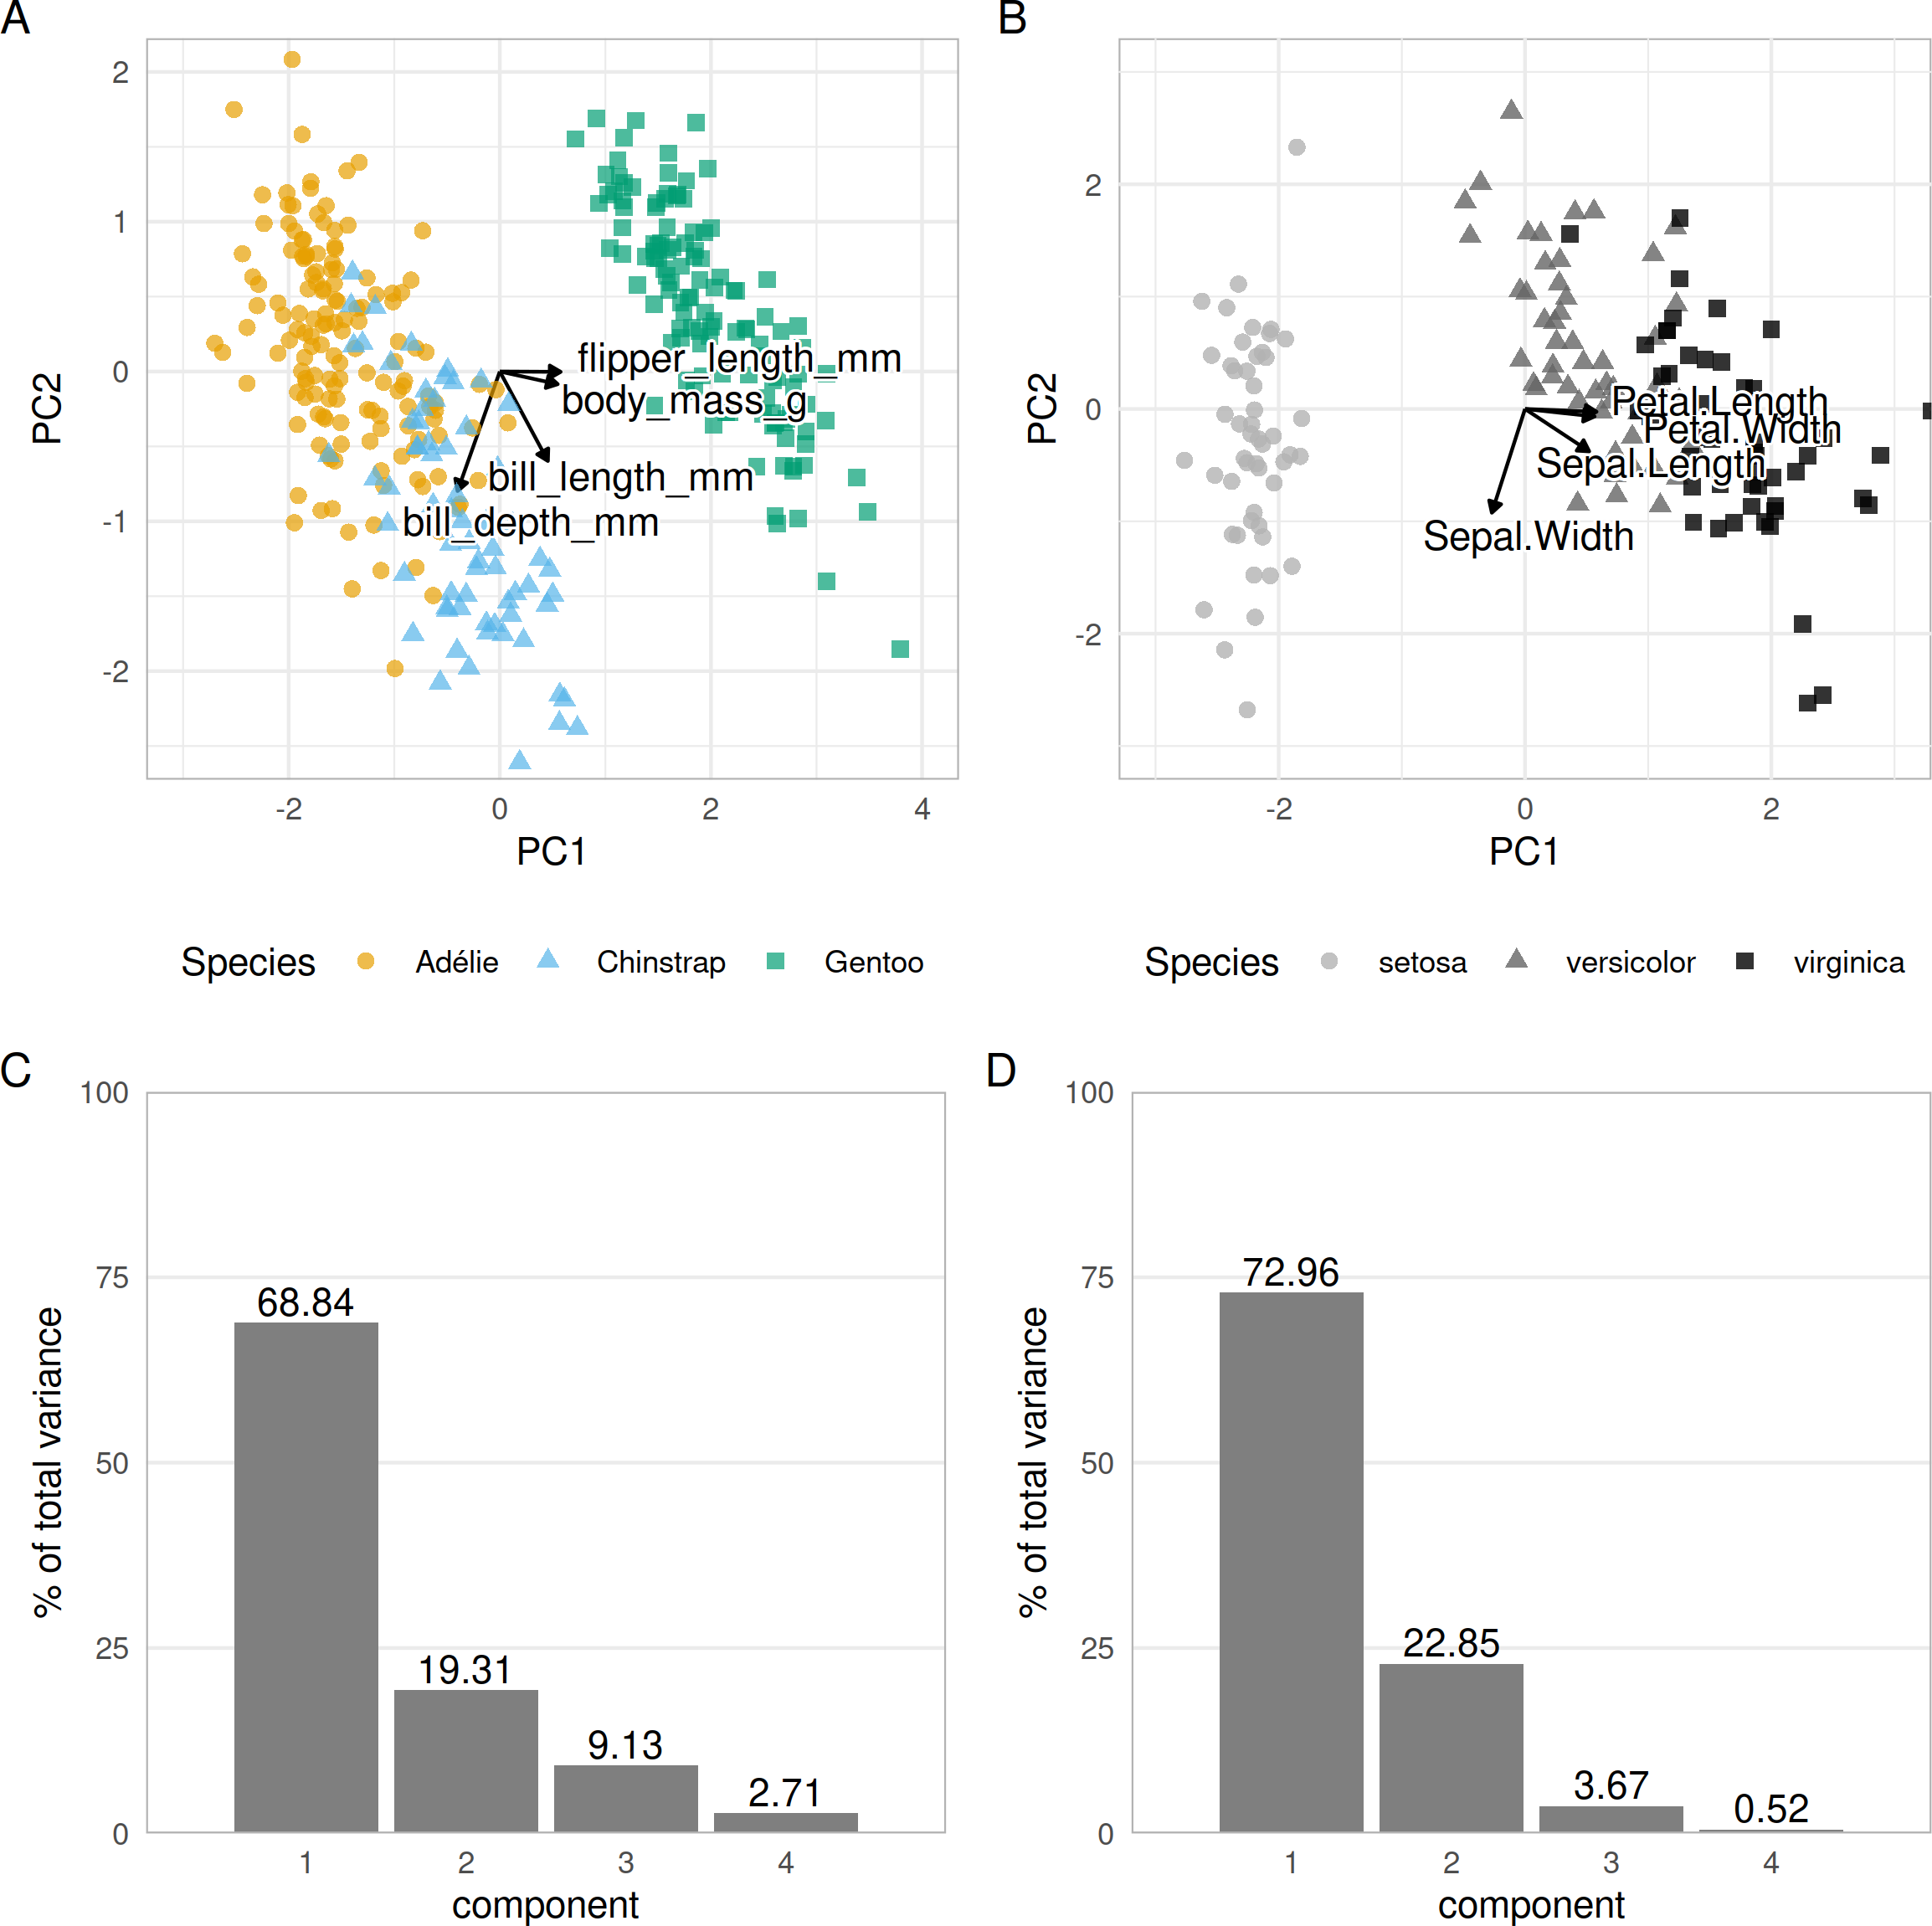
\includegraphics[width=\textwidth]{figs/pca-1} 

}

\caption{Principal component analysis biplots and screeplots for structural size measurements in \textbf{penguins} (A,C) and \textbf{iris} (B,D), revealing similarities in multivariate patterns, variable loadings, and variance explained by each component. For \textbf{penguins}, variables are flipper length (mm), body mass (g), bill length (mm) and bill depth (mm); groups are visualized by species (Adélie = orange circles, Chinstrap = blue triangles, Gentoo = green squares). For \textbf{iris}, variables are petal length (cm), petal width (cm), sepal length (cm) and sepal width (cm); groups are visualized by species (\textit{Iris setosa} = light gray circles, \textit{Iris versicolor} = dark gray triangles, \textit{Iris virginica} = black squares). Values above screeplot columns (C,D) indicate percent of total variance explained by each of the four principal components.}\label{fig:pca}
\end{figure}
\end{Schunk}

\hypertarget{k-means-clustering}{%
\subsubsection{K-means clustering}\label{k-means-clustering}}

Unsupervised clustering by k-means is a common and popular entryway to
machine learning and classification, and again, the \texttt{iris}
dataset is frequently used in introductory examples. The
\texttt{penguins} data provides similar opportunities for introducing
k-means clustering. For simplicity, we compare k-means clustering using
only two variables for each dataset: for \texttt{iris}, petal width and
petal length, and for \texttt{penguins}, bill length and bill depth. All
variables are scaled prior to k-means. Three clusters (\emph{k} = 3) are
specified for each, since there are three species of irises (\emph{Iris
setosa}, \emph{Iris versicolor}, and \emph{Iris virginica}) and penguins
(Adélie, Chinstrap and Gentoo).

K-means clustering with penguin bill dimensions and iris petal
dimensions yields largely distinct clusters, each dominated by one
species (Figure \ref{fig:kmeans}). For iris petal dimensions, k-means
yields a perfectly separated cluster (Cluster 3) containing all 50
\emph{Iris setosa} observations and zero misclassified \emph{Iris
virginica} or \emph{Iris versicolor} (Table \ref{tab:kmeans-tbl}). While
clustering is not perfectly distinct for any penguin species, each
species is largely contained within a single cluster, with little
overlap from the other two species. For example, considering Adélie
penguins (orange observations in Figure \ref{fig:kmeans}A): 147 (out of
151) Adélie penguins are assigned to Cluster 3, zero are assigned to
Cluster 1, and 4 are assigned to the Chinstrap-dominated Cluster 2
(Table \ref{tab:kmeans-tbl}). Only 5 (of 68) Chinstrap penguins and 1
(of 123) Gentoo penguins are assigned to the Adélie-dominated Cluster 3
(Table \ref{tab:kmeans-tbl}).

\begin{Schunk}
\begin{figure}[htbp]

{\centering 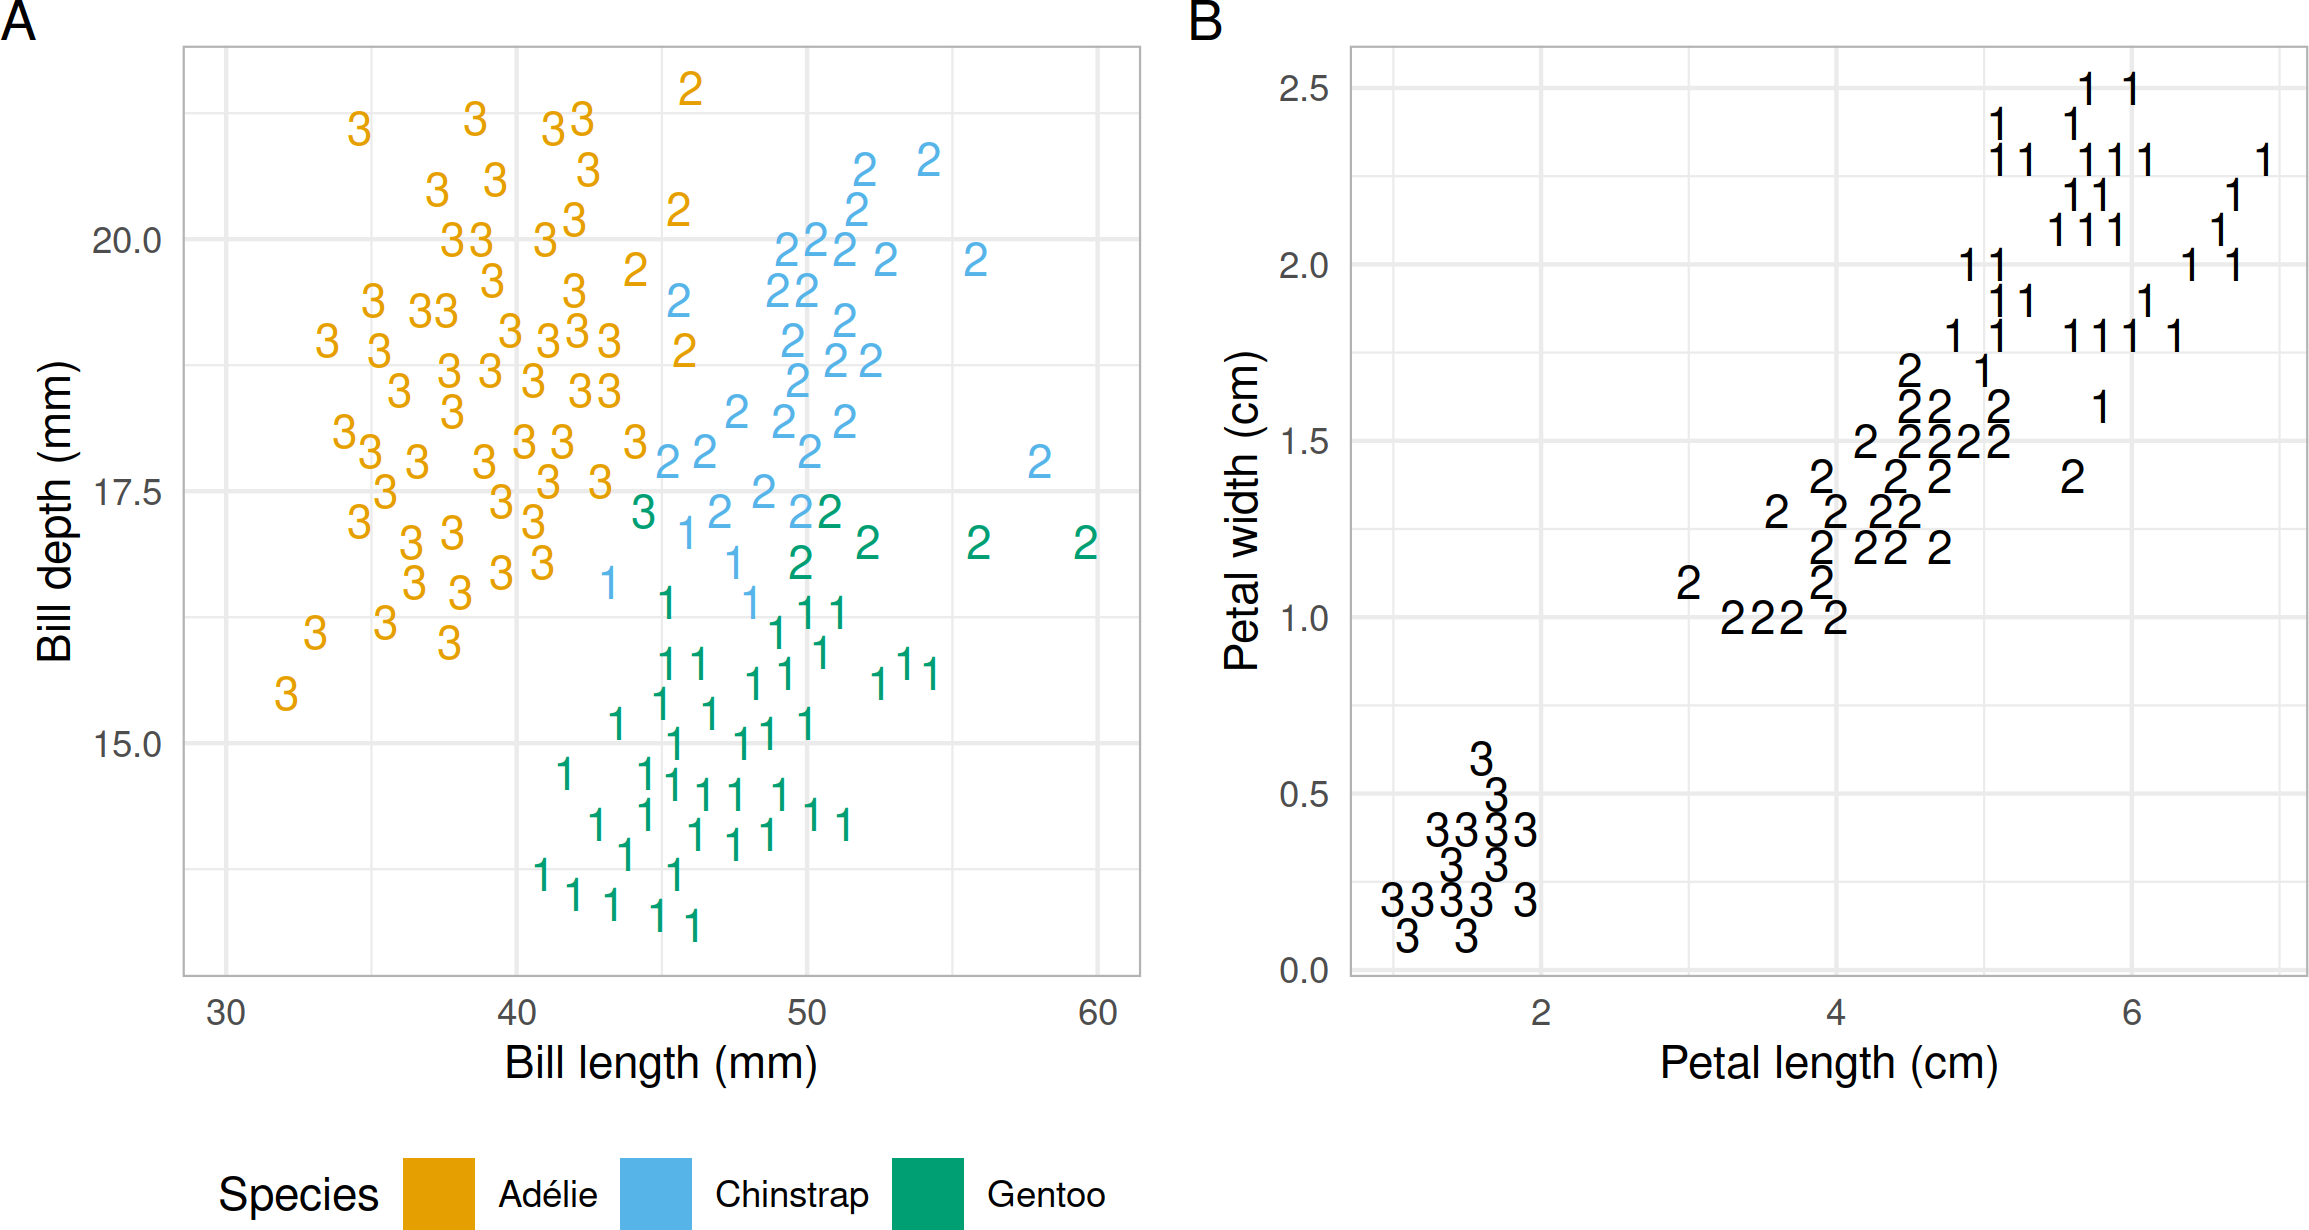
\includegraphics[width=\textwidth]{figs/kmeans-1} 

}

\caption[K-means clustering outcomes for penguin bill dimensions (A) and iris petal dimensions (B)]{K-means clustering outcomes for penguin bill dimensions (A) and iris petal dimensions (B). Numbers indicate the cluster to which an observation was assigned, revealing a high degree of separation between species for both \textbf{penguins} and \textbf{iris}.}\label{fig:kmeans}
\end{figure}
\end{Schunk}

\begin{Schunk}
\begin{table}

\caption{\label{tab:kmeans-tbl}K-means cluster assignments by species based on penguin bill length (mm) and depth (mm), and iris petal length (cm) and width (cm).}
\centering
\begin{tabular}[t]{cccccccc}
\toprule
\multicolumn{4}{c}{Penguins cluster assignments} & \multicolumn{4}{c}{Iris cluster assignments} \\
\cmidrule(l{3pt}r{3pt}){1-4} \cmidrule(l{3pt}r{3pt}){5-8}
Cluster & Adélie & Chinstrap & Gentoo & Cluster & setosa & versicolor & virginica\\
\midrule
1 & 0 & 9 & 116 & 1 & 0 & 2 & 46\\
2 & 4 & 54 & 6 & 2 & 0 & 48 & 4\\
3 & 147 & 5 & 1 & 3 & 50 & 0 & 0\\
\bottomrule
\end{tabular}
\end{table}

\end{Schunk}

\hypertarget{conclusion}{%
\subsection{Conclusion}\label{conclusion}}

Here, we have shown that structural size measurements for Palmer
Archipelago \emph{Pygoscelis} penguins, available as \texttt{penguins}
in the \CRANpkg{palmerpenguins} R package, offer a near drop-in
replacement for \texttt{iris} in a number of common use cases for data
science and statistics education including exploratory data
visualization, linear correlation and regression, PCA, and clustering by
k-means. In addition, teaching and learning opportunities in
\texttt{penguins} are increased due to a greater number of variables,
missing values, unequal sample sizes, and Simpson's Paradox examples.
Importantly, the \texttt{penguins} dataset encompasses real-world
information derived from several charismatic marine predator species
with regional breeding populations notably responding to environmental
change occurring throughout the Western Antarctic Peninsula region of
the Southern Ocean (see \citet{bestelmeyer_analysis_2011},
\citet{gorman_ecological_2014}, \citet{gorman_population_2017},
\citet{gorman_advancing_2021}). Thus, the \texttt{penguins} dataset can
facilitate discussions more broadly on biodiversity responses to global
change - a contemporary and critical topic in ecology, evolution, and
the environmental sciences.

\hypertarget{penguins-data-processing}{%
\subsection{Penguins data processing}\label{penguins-data-processing}}

Data in the \texttt{penguins} object have been minimally updated from
\texttt{penguins\_raw} as follows:

\begin{itemize}
\tightlist
\item
  All variable names are converted to lower snake case (e.g.~from
  \texttt{Flipper\ Length\ (mm)} to \texttt{flipper\_length\_mm})
\item
  Entries in \texttt{species} are truncated to only include the common
  name (e.g.~``Gentoo'', instead of ``gentoo penguin (\emph{Pygoscelis
  papua})'')
\item
  Recorded sex for penguin N36A1, originally recorded as ``.'', is
  updated to \texttt{NA}
\item
  \texttt{culmen\_length\_mm} and \texttt{culmen\_depth\_mm} variable
  names are updated to \texttt{bill\_length\_mm} and
  \texttt{bill\_depth\_mm}, respectively
\item
  Class for categorical variables (\texttt{species}, \texttt{island},
  \texttt{sex}) is updated to factor
\item
  Variable \texttt{year} was pulled from clutch observations
\end{itemize}

\hypertarget{summary-of-the-penguins_raw-dataset}{%
\subsection{\texorpdfstring{Summary of the \texttt{penguins\_raw}
dataset}{Summary of the penguins\_raw dataset}}\label{summary-of-the-penguins_raw-dataset}}

\begin{Schunk}

\begin{tabular}{ll}
\toprule
Feature & penguins\_raw\\
\midrule
Year(s) collected & 2007 - 2009\\
Dimensions (col x row) & 17 x 344\\
Documentation & complete metadata\\
Variable classes & character (9), Date (1), numeric (7)\\
Missing values? & yes (n = 336; 5.7\%)\\
\bottomrule
\end{tabular}

\end{Schunk}

\hypertarget{palmerpenguins-for-other-programming-languages}{%
\subsection{palmerpenguins for other programming
languages}\label{palmerpenguins-for-other-programming-languages}}

\textbf{Python:} Python users can load the palmerpenguins datasets into
their Python environment using the following code to install and access
data in the
\href{https://pypi.org/project/palmerpenguins/}{palmerpenguins Python
package}:

\begin{verbatim}
pip install palmerpenguins
from palmerpenguins import load_penguins
penguins = load_penguins()
\end{verbatim}

\textbf{Julia:} Julia users can access the penguins data in the
\textbf{PalmerPenguins.jl} package. Example code to import the penguins
data through \textbf{PalmerPenguins.jl} (more information on
\textbf{PalmerPenguins.jl} from David Widmann can be found
\href{https://github.com/devmotion/PalmerPenguins.jl}{here}):

\begin{verbatim}
julia> using PalmerPenguins
julia> table = PalmerPenguins.load()
\end{verbatim}

\textbf{TensorFlow:} TensorFlow users can access the penguins data in
TensorFlow Datasets. Information and examples for \textbf{penguins} data
in TensorFlow can be found
\href{https://www.tensorflow.org/datasets/catalog/penguins}{here}.

\hypertarget{acknowledgements}{%
\subsection{Acknowledgements}\label{acknowledgements}}

All analyses were performed in the R language environment using version
4.1.2 \citep{R-base}. Complete code for this paper is shared in the
Supplemental Material. We acknowledge the following R packages used in
analyses, with gratitude to developers and contributors:

\begin{itemize}
\tightlist
\item
  \CRANpkg{GGally} \citep{R-GGally}: for pairs plots
\item
  \CRANpkg{ggiraph} \citep{R-ggiraph}: for interactive \CRANpkg{ggplot2}
  graphics
\item
  \CRANpkg{ggplot2} \citep{R-ggplot2}: for data visualizations
\item
  \CRANpkg{kableExtra} \citep{R-kableExtra}: for finalized tables
\item
  \CRANpkg{paletteer} \citep{R-paletteer}: for the Okabe Ito color
  palette, provided by the \CRANpkg{colorblindr} package
\item
  \CRANpkg{patchwork} \citep{R-patchwork}: for compound figures
\item
  \CRANpkg{plotly} \citep{R-plotly}: for interactive graphics
\item
  \CRANpkg{recipes} \citep{R-recipes} and \CRANpkg{broom}
  \citep{R-broom}: for modeling
\item
  \CRANpkg{shadowtext} \citep{R-shadowtext}: to add a background color
  to text labels
\item
  \CRANpkg{tidyverse} \citep{tidyverse2019}: for data import and
  cleaning
\end{itemize}

\bibliography{penguins.bib}

\address{%
Allison M. Horst\\
University of California Santa Barbara\\%
Bren School of Environmental Science and Management\\ Santa Barbara, CA
93106-5131\\
%
%
%
\href{mailto:ahorst@ucsb.edu}{\nolinkurl{ahorst@ucsb.edu}}%
}

\address{%
Alison Presmanes Hill\\
Voltron Data\\%
\\
%
%
%
\href{mailto:apreshill@gmail.com}{\nolinkurl{apreshill@gmail.com}}%
}

\address{%
Kristen B. Gorman\\
University of Alaska Fairbanks\\%
College of Fisheries and Ocean Sciences\\ 2150 Koyukuk Drive\\ 245
O'Neill Building\\ Fairbanks, AK 99775-7220\\
%
%
%
\href{mailto:kbgorman@alaska.edu}{\nolinkurl{kbgorman@alaska.edu}}%
}
